\paragraph{}
	Dans cette partie, nous allons décrire en détail les différentes spécifications propres à notre projet. En premier lieu, nous commencerons par détailler les spécifications fonctionnelles en rappelant les diverses fonctionnalités attendues ainsi que nos objectifs. Nous appuierons nos explications à l'aide de maquette d'une étude des cas d'utilisation. En second lieu, nous présenterons les spécifications techniques de notre projet.

\section{Spécifications fonctionnelles}
\subsection{Présentation de la problématique}

	\paragraph{}
		Le but de ce projet d'approfondissement et d'ouverture est de concevoir une application Android permettant de fournir des informations ainsi que des conduites à tenir pour assister les touristes et les résidents étrangers en France. Les informations contenues au sein de cette dernière devront pouvoir transiter en format numérique aussi bien sur SmartPhone que sur tablette. L'application sera proposée à des utilisateurs de différentes nationalités dont le niveau de connaissances informatiques est très hétérogène c'est pourquoi elle devra être graphique, lisible et simple d'utilisation.
\subsection{Objectifs}
	
	\paragraph{}
		Nous allons maintenant présenter les différents objectifs que notre application devra atteindre. Ces derniers sont les suivants :
\begin{itemize}
	\item Fournir les informations appropriées en fonction de la situation du touriste.
	\item Déclencher les conduites à tenir en cas d'urgence (appels téléphoniques vers différents services).
	\item Être multilingue.
	\item Supporter l'ajout de nouvelles fiches d'informations fournies par la gendarmerie ou langues.
	\item Avoir un module de géolocalisation permettant de guider le touriste vers l'adresse désignée (ambassade, consulat, police, gendarmerie ...).
	\item Être graphique et très simple/rapide d'utilisation.
\end{itemize}
\subsection{Fonctionnalités}

\paragraph{}
	Nous allons maintenant détailler les différentes fonctionnalités qui feront parties intégrantes de notre projet.
	
\subsubsection{Conseils de prévention}
	\paragraph{}
		L'application devra permettre de fournir à l'utilisateur des informations appropriées en fonction de sa situation.Par exemple, elles peuvent concerner les transports en commun, les lieux publics, les hôtels ou encore les urgences. Ces informations auront pour objectif de conseiller un touriste étranger en France sur la conduite à adopter et la manière d'appréhender les choses lorsque celui-ci se trouve dans une situation particulière. Ces conseils sont fournis sous forme de fiche au format odt par la gendarmerie. De plus, celle-ci souhaite pouvoir ajouter de nouvelles informations lorsqu'elle le désire. Cependant, les connaissances informatique du client étant limitées, l'application devra permettre un ajout simplifié de ces informations. Par exemple par simple dépôt d'une fiche au bon format dans un dossier. Les situations seront symbolisées sous forme de liste de pictogrammes explicites auxquels seront adjoints des mots clés.

\subsubsection{Contacts}
	\paragraph{}
			L'application devra donner la possibilité à l'utilisateur d'accéder à une liste de contacts à appeler en cas d'urgence. Cette liste contiendra des numéros tels que ceux de la gendarmerie/police, des urgences, des pompiers ... Cette liste permettra de rediriger l'utilisateur sur son composeur téléphonique avec le numéro correspondant au contact qu'il souhaite appeler. Ainsi, celui-ci aura toujours le choix de confirmer ou d'annuler l'appel.
			
\subsubsection{Géolocalisation}
	\paragraph{}
			L'application devra contenir un module de géolocalisation et de navigation permettant de guider l'utilisateur vers la destination de son choix. Elle proposera une liste de destinations pouvant être utiles en fonction de la situation du touriste comme la gendarmerie, le consulat ou l'hôpital. Cette fonctionnalité aura pour objectif de renvoyer l'utilisateur sur Google Maps avec une recherche pré-effectuée pointant sur la direction qu'il aura choisi.
			
\subsubsection{Profil}
	\paragraph{}
			L'application devra permettre à l'utilisateur de pouvoir écrire ses informations personnelles ainsi que que les remarques médicales le concernant. Ces informations pourront être utilisées en cas d'urgence ou pour lister les différents problèmes concernant l'utilisateur.
			
\subsubsection{Multilingue}
	\paragraph{}
			L'application étant proposée à des touristes ou résidents étranger en France, celle-ci devra être multilingue. Les différents menus, listes de contacts et destinations seront donc traduits dans différentes langues. Les fiches de conseils devront également être traduites dans différentes langues. Elle devra proposer à l'utilisateur de choisir sa nationalité lors de sa première utilisation de l'application. De plus, elle devra également lui permettre de pouvoir modifier son choix et donc de changer de langue à tout moment.
			
			
\subsection{Cas d'utilisation}

Le diagramme présent sur la figure \ref{casUtilisations} permet de représenter les différents cas d'utilisation de l'application.
	
\begin{figure}[!h]
	\begin{center}
	
		\includegraphics[scale=0.6]{img/casUtilisations.png}
	    \caption{Diagramme de Cas d'Utilisation}
	    \label{casUtilisations} 
	
	\end{center}
\end{figure}

\newpage
\subsection{Maquette}

Les images \ref{maquette1} et \ref{maquette2} représentent la maquette permettant de décrire le cahier des charges et les spécifications d'interface qui ont été fourni pour la réalisation de l'application.

\begin{figure}[!h]
	\begin{center}
		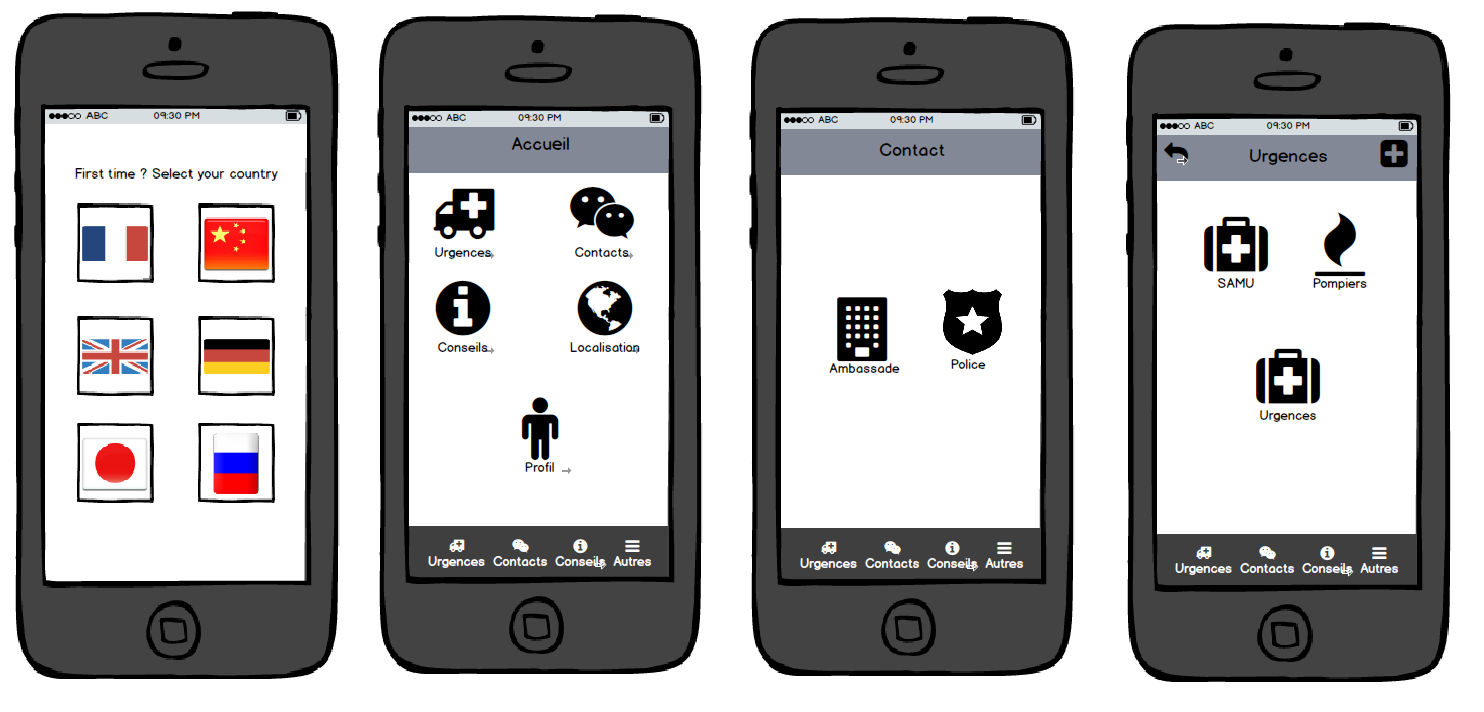
\includegraphics[scale=0.45]{img/maquette1.png}
		\caption{Maquette de l'application}
		\label{maquette1} 
	\end{center}
\end{figure}

\begin{figure}[!h]
	\begin{center}
		
		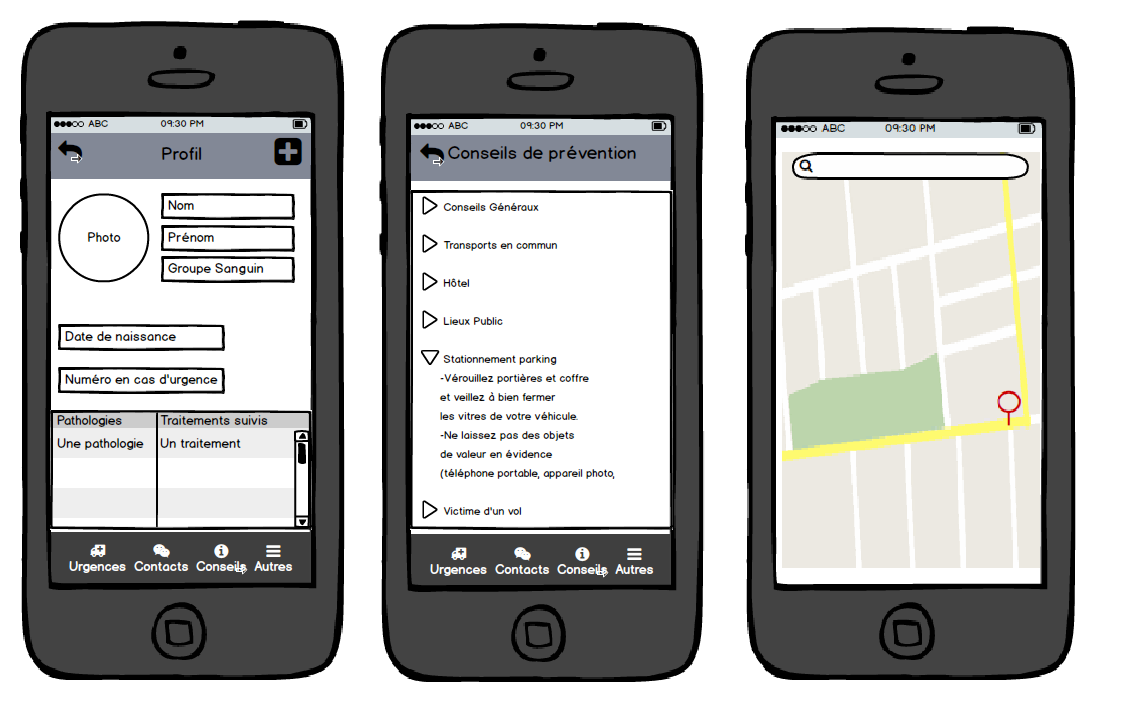
\includegraphics[scale=0.5]{img/maquette2.png}
		\caption{Maquette de l'application : }
		\label{maquette2} 
		
	\end{center}
\end{figure}

\section{Spécifications techniques}
\subsection{Spécifications opérationnelles}

\subsubsection{Caractéristiques techniques}
	L'application sera fonctionnelle sous les systèmes d'exploitation mobile Android en version 4.0 minimum et IOS en version ?. Celle-ci devra être fluide et adaptée à une utilisation tactile. Elle sera proposée à des  utilisateurs ayant des nationalités différentes c'est pourquoi elle devra être lisible et graphique.
	Cette application sera off-line c'est-à-dire sans échange de données direct. Dans le but d'utiliser le module de géolocalisation elle devra faire appel à une application tierce, Google Maps. En outre, elle sera responsive et donc en mesure de s'adapter à différents écrans.

\subsubsection{Permissions}

	L'application nécessitera plusieurs permissions dans l'optique que l'utilisateur puisse profiter pleinement de toutes ses fonctionnalités. Les permissions requises sont les suivantes : 
	\begin{itemize}
		\item \texttt{android.permission.CALL\_PHONE} Autorise l'application à rediriger l'utilisateur sur le composeur téléphonique en lui laissant le choix de confirmer ou non l'appel.
		\item \texttt{android.permission.READ\_EXTERNAL\_STORAGE} Autorise l'application à lire du contenu externe stocké sur le téléphone.
		\item \texttt{android.permission.ACCESS\_COARSE\_LOCATION} Autorise l'application à utiliser les fonctions de géolocalisation approximative.
		\item \texttt{android.permission.ACCESS\_FINE\_LOCATION} Autorise l'application à utiliser les fonctions de géolocalisation de haute précision.
	\end{itemize}
	
\subsection{Outils technologiques}

	\paragraph{}
		Comme nous l'avons expliqué ci-dessus l'application devra être en mesure de fonctionner sous Android et IOS. Cette dernière a déjà été développé en natif sous Android Studio pour le système d'exploitation Android. N'ayant aucune nouvelle de notre client, le choix qui a été fait était de concevoir différente version de l'application afin de pouvoir laisser le client choisir celle qui lui convenait le mieux. Ainsi, nous avons décidé de nous séparer en deux équipes, l'une travaillant sur le développement natif de l'application IOS et l'autre travaillant sur la réalisation d'une application multi plate-forme.
		
	\paragraph{}
		La première équipe composée de Darchen Gautier et Judic Romain a développé une application IOS native à l'aide du langage de programmation Swift et de l'environnement de développement xCode sous macOS. Plus d'informations sur cette partie du projet seront disponibles dans le rapport associé.
		
	\paragraph{}
		En ce qui me concerne, j'ai travaillé sur la réalisation de l'application multi plate-forme. Afin de procéder à cela je me suis tourner vers le développement d'une application hybride, connue pour être bien plus efficace et moins coûteuse en ressource que les applications web cross-platform. Cette application a été réalisée à l'aide du framework \emph{Xamarin} et du langage de programmation \emph{C\#}. Xamarin est disponible gratuitement sous Windows en installant un plugin pour Microsoft Visual Studio ou alors sous MacOS via Xamarin Studio. Ici, l'application a été développée à l'aide de Xamarin Studio. 	 
		   	
